\documentclass[
	12pt, % Schriftgröße
	DIV=10,
	ngerman, %für Umlaute, Silbnetrennung etc.
	a4paper, % Papierformat
	oneside, % einseitiges Dokument
	titlepage, % es wird eine Titelseite verwendet
	parskip=half, % Abstand zwischen Absätzen (halbe Zeile)
	BCOR=10mm,		% Bindekorrektur links: 10mm
	%headings=normal, % Größe der Überschriften verkleinern
	listof=totoc, % Verzeichnisse im Inhaltsverzeichnis aufführen
	listof=entryprefix, % enable prefix for toc entries, e.g. "Abb. "
	bibliography=totoc, % Literaturverzeichnis im Inhaltsverzeichnis aufführen
	index=totoc, % Index im Inhaltsverzeichnis aufführen
	%captions=tableheading, % place table captions above table
	final, % Status des Dokuments (final/draft)
	hidelinks, %entfernt hässliche Boxen
	numbers=noenddot, % entfernt Punkte hinter Kapitelzahlen
	hyphens,
	]{scrreprt}%{scrartcl}

%TODO: create variables and implement syntax like \art{T1000}
\newcommand{\art}{Studienarbeit} %feminin
\newcommand{\titel}{Programmentwurf Mobile Computing}
\newcommand{\untertitel}{Kalenderapp}

\newcommand{\studiengang}{Elektrotechnik und Informationstechnik}
\newcommand{\studienfach}{Elektrotechnik und Informationstechnik} %Wird nur für Bachelordeckblatt benötigt.

\newcommand{\hochschule}{Dualen Hochschule Baden-Württemberg} %An der ...
\newcommand{\campus}{Center of Advanced Studies}
\newcommand{\abgabeort}{Heilbronn}

\newcommand{\autor}{Lukas Renz}

\newcommand{\jahrgang}{2024}
\newcommand{\matrikelnr}{4681850}
\newcommand{\kurs}{ET2022} % Nicht verwendet
\newcommand{\bearbeitungszeitraum}{November 2024 bis Dezember 2024}
\newcommand{\gutachter}{Prof. Dr. Kai Becher} % Nicht verwendet

\newcommand{\dateiname}{Programmentwurf} % Nicht verwendet


\newcommand{\ladeliteratur}{
\addbibresource{Literatur.bib}
%\addbibresource{WeitereLiteratur.bib}
}
% Include from Einstellungen.tex
\title{\titel}
\author{\autor}
%\date{\today} % set date for default title page (\maketitle) -- not used with custom title page

\usepackage[english, main=ngerman]{babel} % set language -- ngerman is default, english needed for acro

\usepackage{scrhack} % improves compatibility with KOMA

\usepackage{subcaption} % Für Subfiguren

% handle encoding
\usepackage[T1]{fontenc} % use 256-glyph font (e.g. makes "ü" a glyph) enables copy-pasting of umlauts
\usepackage[utf8]{inputenc} % allow all UTF-8 characters in source

% page geometry
\usepackage[left=2.50cm, right=2.50cm, top=2.50cm, bottom=3.10cm]{geometry}	% define margins
\usepackage{pdflscape} % allow landscape pages
\renewcommand*{\chapterheadstartvskip}{\vspace*{.7\baselineskip}}% reduce chapter headings margin
\setcounter{secnumdepth}{3} % number subsubsections
\setcounter{tocdepth}{2} %subsections im toc anzeigen
\setuptoc{toc}{totoc} % add toc to toc

\usepackage[onehalfspacing]{setspace} % line spacing 1.5
\usepackage{microtype} % improve typesetting -> avoid over- / underfull boxes
\usepackage{textcomp} % defines additional symbols (see: https://ctan.org/pkg/textcomp ??)
% Hurenkinder und Schusterjungen verhindern
% http://projekte.dante.de/DanteFAQ/Silbentrennung -- link deprecated!
\clubpenalty = 10000 % schließt Schusterjungen aus (Seitenumbruch nach der ersten Zeile eines neuen Absatzes)
\widowpenalty = 10000 % schließt Hurenkinder aus (die letzte Zeile eines Absatzes steht auf einer neuen Seite)
\displaywidowpenalty=10000


% Font
\usepackage{noto}
%\usepackage[scaled]{helvet}
%\usepackage{lmodern}

\usepackage{etoolbox} %Untersützt ifstrempty

% footnotes
\usepackage{chngcntr} 
\counterwithout{footnote}{chapter} % make footnotes not reset at the beginning of a chapter
\renewcommand{\thempfootnote}{\arabic{mpfootnote}} % number footnotes
\usepackage[perpage, hang, multiple, stable]{footmisc} % add footnote stuff

\usepackage{afterpage} % allows control over float placement (see: https://www.ctan.org/pkg/afterpage)


% math support
\usepackage{amsmath} % math macros like \hat
\usepackage{amsfonts}
\usepackage{amssymb}

% units
\usepackage[locale=DE]{siunitx} % adds \qty and \unit
\DeclareSIUnit[qualifier-mode=combine]\dBm{\dB\of{m}}


\usepackage{lipsum} % Dummytext
\usepackage{blindtext}
\blindmathtrue

 % colors
 \usepackage{color, colortbl}
 %Farbdefinition von hellgrau
 \definecolor{light-gray}{gray}{0.75}
 \definecolor{lightgray}{rgb}{.9,.9,.9}
 \definecolor{darkgray}{rgb}{.4,.4,.4}
 \definecolor{purple}{rgb}{0.65, 0.12, 0.82}
 \definecolor{darkgreen}{RGB}{0, 238, 0}
 \definecolor{blue}{RGB}{44, 111, 235}
 %%%VISUAL STUDIO COLORS
 \definecolor{VSblue}{RGB}{44, 111, 235}
 \definecolor{VSstringred}{RGB}{163, 21, 21}
 \definecolor{VScitrine}{rgb}{0.89, 0.82, 0.04}
 \definecolor{VSblack}{rgb}{0.0, 0.0, 0.0}
 \definecolor{VSgreencomments}{rgb}{0,0.5,0}
 \definecolor{VSclassGreen}{RGB}{0, 125, 154}
 
 \usepackage[dvipsnames,table,xcdraw]{xcolor} % needs to be loaded before pgfplots!


%floats
\usepackage{float}
\addto\extrasngerman{\let\subsectionautorefname\sectionautorefname 	\let\subsubsectionautorefname\sectionautorefname} %Displays sub- and subsubsection as section in \autoref


\usepackage[
	%format=hang, justification=justified,									% format option 1: indented text,	label normal,	separated with colon,	justification
	format=plain, justification=justified, labelfont=bf, labelsep=quad, 	% format option 2: no indents,		label bold,		separated with tab,		justification
	singlelinecheck=true % center captions if they fit into a single line 
	]{caption}
\usepackage{subcaption} % adds caption support for subfigures
%\captionsetup[table]{position=above, aboveskip=4pt}%, belowskip=6pt} % should place the caption of tables above the table. Does not work!

%tables
\usepackage{booktabs} % make nice tables
\usepackage{multirow}
\usepackage{tabularx} % add support for line wrapping in tabels

\newcolumntype{P}[1]{>{\raggedright\arraybackslash}p{#1}}
\newcolumntype{L}{>{$}l<{$}} % math-mode version of "l" column type

\renewcommand{\arraystretch}{2}
\setlength{\tabcolsep}{5mm}
\usepackage{array}% in the preamble

%figures
\usepackage[pdftex]{graphicx}		
\graphicspath{{img/}}
\usepackage{wrapfig} % allow placement of figures in text (wrap text around figure)

\usepackage{flafter} % make sure figures are placed after declaration

% TikZ/PGF

\usepackage{tikz}
\usepackage{pgffor} % foreach loops
\usepackage{pgfplots}
\usepackage{circuitikz}

% externalize pgf plots
\usepgfplotslibrary{external}
\tikzexternalize
\pgfplotsset{
	width=15cm,
	compat=1.18,
	/pgf/number format/.cd,
	use comma,
	1000 sep={ }
}



\usepackage{tcolorbox} % makes colorful boxes (for examples and such)

% listings
\usepackage{listings}
\usepackage{listings-ext}
\lstset{%
	%language=[Sharp]C,			% Standardsprache des Quellcodes
	%backgroundcolor=\color{lightgray}, %Hintergrundfarbe von CODE
	numbers=left,			% Zeilennummern links
	stepnumber=1,			% Jede Zeile nummerieren.
	numbersep=5pt,			% 5pt Abstand zum Quellcode
	numberstyle=\tiny,		% Zeichengrösse 'tiny' für die Nummern.
	breaklines=true,		% Zeilen umbrechen wenn notwendig.
	breakautoindent=true,	% Nach dem Zeilenumbruch Zeile einrücken.
	postbreak=\space,		% Bei Leerzeichen umbrechen.
	tabsize=2,				% Tabulatorgrösse 2
	basicstyle=\ttfamily\footnotesize, % Nichtproportionale Schrift, klein für den Quellcode
	showspaces=false,		% Leerzeichen nicht anzeigen.
	showstringspaces=false,	% Leerzeichen auch in Strings ('') nicht anzeigen.
	extendedchars=true,		% Alle Zeichen vom Latin1 Zeichensatz anzeigen.
	captionpos=b,			% sets the caption-position to bottom
	%backgroundcolor=\color{ListingBackground}, % Hintergrundfarbe des Quellcodes setzen.
	xleftmargin=0pt,		% Rand links
	xrightmargin=0pt,		% Rand rechts
	frame=single,			% Rahmen an
	frameround=ffff,
	rulecolor=\color{darkgray},	% Rahmenfarbe
	%fillcolor=\color{ListingBackground},
	keywordstyle=\color[rgb]{0.133,0.133,0.6},
	commentstyle=\color[rgb]{0.133,0.545,0.133},
	stringstyle=\color[rgb]{0.627,0.126,0.941}
} % uses textcomp
\renewcommand\lstlistingname{Codeausschnitt}
\renewcommand\lstlistlistingname{Quellcodeverzeichnis}

%Umlaute und Sonderzeichen im listings erlauben
\lstset{literate=%
	{Ö}{{\"O}}1
	{Ä}{{\"A}}1
	{Ü}{{\"U}}1
	{ß}{{\ss}}2
	{ü}{{\"u}}1
	{ä}{{\"a}}1
	{ö}{{\"o}}1
	{&}{{\&}}1
}


\usepackage{enumitem} % allows control about enumeration format

% acronyms
\usepackage{acro}

\NewAcroTemplate{shortLong}{%
	\acroiffirstTF{%
		\acrowrite{short}%
		#2%
		\acspace%
		(\ifstrempty{#2}{}{\acrowrite{short}: }%
		\acroifT{foreign}{\acrowrite{foreign}, }%
		\acrowrite{long}%
		\acroifT{alt}{ \acrotranslate{or} \acrowrite{alt}})%
	}%
	{\acrowrite{short}#2}%
}

\RenewAcroCommand\ac{m O{}}{\UseAcroTemplate{shortLong}[2]{#1}{#2}}
\RenewAcroCommand\acp{m O{}}{\acroplural\UseAcroTemplate{shortLong}[2]{#1}{#2}}
\RenewAcroCommand\iac{m O{}}{\acroindefinite\UseAcroTemplate{shortLong}[2]{#1}{#2}}
\RenewAcroCommand\Ac{m O{}}{\acroupper\UseAcroTemplate{shortLong}[2]{#1}{#2}}
\RenewAcroCommand\Acp{m O{}}{\acroplural\acroupper\UseAcroTemplate{shortLong}[2]{#1}{#2}}
\RenewAcroCommand\Iac{m O{}}{\acroupper\acroindefinite\UseAcroTemplate{shortLong}[2]{#1}{#2}}

\acsetup{
	first-style=shortLong,
	trailing/activate={dash}, 
	make-links=true,
	list/heading=addchap, % format table of acronyms (toa) as chapter* and add tot toc (\addchap of KOMA)
	list/name= {Abkürzungsverzeichnis} % make table-of-commands style uniform
}


%bibliography
\usepackage[style=ieee, %authortitle, %Zitierstil
	bibstyle=ieee, %authortitle,
	language=ngerman, %Quellen auf Deutsch
	hyperref=true, %Anklickbare Referenzen
	natbib=true, 
	backend=biber, 
	pagetracker=true, %ebd. bei wiederholten Angaben
	bibencoding=utf8,
	backrefstyle=three+, % fasst Seiten zusammen, z. B S. 2f, 6ff, 7-10
	date=short, %Datumsformat
	bibwarn=true]{biblatex}

\renewcommand*{\labelalphaothers}{\textsuperscript{+}} % handle multiple authors
	
\usepackage[babel,german=guillemets]{csquotes} % select quotes for bibliography
\setlength{\bibitemsep}{1em}     % Abstand zwischen den Literaturangaben
\setlength{\bibhang}{2em}        % Einzug nach jeweils erster Zeile
% include bib files (configured in Einstellungen.tex)
\ladeliteratur

\setcounter{biburllcpenalty}{7000}
\setcounter{biburlucpenalty}{8000}

				
% kopf und fußzeile
\usepackage[headsepline, footsepline, plainheadsepline, plainfootsepline]{scrlayer-scrpage}		% linie aktivieren für "headings" und "plain" seiten
\automark{chapter}		% aktivieren das "chapter" und "section" oeben angezeigt werden kann
\automark*{section}

\setlength{\headheight}{35pt}			% header abstand
\setlength{\footheight}{\baselineskip}	% footer abstand

\clearpairofpagestyles

% Der "*" macht, dass hier konfigurierte Einstellungen auch für "plain"-Seiten gelten
%\ihead*{\vspace*{-0.0cm}\includegraphics[height=1cm, width=0.3\textwidth, keepaspectratio, angle=0]{\firmenlogo}}	% firmenlogo etwas runtersetzen, da komisch formatiert
\chead{\normalfont \headmark}		% "chapter" und "section" oben mittig anzeigen
\ohead*{
\includegraphics[height=2cm, angle=0]{img/dhbwlogo.jpg}}	% DHBW Logo

%\ifoot*{\scriptsize \normalfont Autor: \autor}	% \scriptsize -> kleine Schriftgröße      \normalfont -> Nicht Kursiv
\cfoot*{\scriptsize \normalfont Datum: \today}  % Autor Links, Datum mitte, Seitenzahl rechts
\ofoot{\pagemark}

\renewcommand*{\chapterpagestyle}{headings}		% pagestyle von der ersten seite eines kapitels ändern
\renewcommand*{\titlepagestyle}{plain}		% pagestyle von der titelseite ändern (funktioniert hier nicht, da kein "richtiger" titel nach koma-skript gesetzt wird)

\renewcaptionname{ngerman}{\bibname}{Literaturverzeichnis} % change name of bibliography

% Formelverzeichniss
\DeclareNewTOC[
	tocentryindent=0pt,
    tocentrynumwidth=2em,
	type=equation,
	name={Gl.},
	types=equations,
	listname={Formelverzeichnis},
]{equ}
\newcommand{\addequations}[2][\theequation]{%
	\addxcontentsline{equ}{equation}[{#1}]{\kern 1em #2}%
}


\usepackage{url} % hyphenate urls - needs to be loaded before hyperref-package!
\usepackage{bookmark} %nur ein latex-Durchlauf für die Aktualisierung von Verzeichnissen nötig

% allow hyper links in pdf
\usepackage{hyperref}
\hypersetup{
	pdftitle={\titel},
	pdfauthor={\autor},
	pdfsubject={\art},
	pdfcreator={pdflatex, LaTeX with KOMA-Script},
	pdfpagemode=UseOutlines, 		% Beim Oeffnen Inhaltsverzeichnis anzeigen
	pdfdisplaydoctitle=true, % Dokumenttitel statt Dateiname anzeigen.
	breaklinks=true		
}



\newenvironment{symboltable}{
	\par
	\let\stretchbuf\arraystretch
	\renewcommand{\arraystretch}{1}
	\tabularx{\textwidth}{rX}
}{
	\endtabularx
	\renewcommand{\arraystretch}{\stretchbuf}
	\par
}
\lstloadlanguages{PHP,Python,Java,C,C++,bash,[Sharp]C,HTML} %weitere Sprachen: http://texdoc.net/texmf-dist/doc/latex/listings/listings.pdf auf Seite 13
\lstdefinestyle{Csharp} {language=[Sharp]C} %[] kann in listingdefinition nicht verwendet werden
\lstdefinelanguage{JavaScript}{
  keywords={typeof, new, true, false, catch, function, return, null, catch, switch, var, if, in, while, do, else, case, break, script, type},
  keywordstyle=\color{blue}\bfseries,
  ndkeywords={class, export, boolean, throw, implements, import, this},
  ndkeywordstyle=\color{darkgray}\bfseries,
  identifierstyle=\color{black},
  sensitive=false,
  comment=[l]{//},
  morecomment=[s]{/*}{*/},
  commentstyle=\color{purple}\ttfamily,
  stringstyle=\color{red}\ttfamily,
  morestring=[b]',
  %morestring=[b]"
}


\lstdefinelanguage{Gherkin}{
	morekeywords = {
		Given,
		When,
		Then,
		And,
		Scenario,
		Feature,
    But,
    but,
		Background,
		Scenario Outline,
    Examples,
    Example,
    Rule
	},
	sensitive=true,
	morecomment=[l]{\#},
	morestring=[b]",
	morestring=[b]'
}

\definecolor{gray}{rgb}{0.4,0.4,0.4}
\definecolor{darkblue}{rgb}{0.0,0.0,0.6}
\definecolor{cyan}{rgb}{0.0,0.6,0.6}

\lstdefinelanguage{XML}
{
  morestring=[b]",
  morestring=[s]{>}{<},
  morecomment=[s]{<?}{?>},
  stringstyle=\color{black},
  identifierstyle=\color{darkblue},
  keywordstyle=\color{cyan},
  morekeywords={xmlns,version,type}% list your attributes here
}

\lstdefinelanguage{CS}{
  keywords=[1]{typeof, new, true, false, catch, function, return, null, catch, switch, var, if, in, while, do, else, case, break, script, type, public, private, class, interface, int, string, bool, this, throw, foreach, for, static, extern,void,object, float, double, ref, out,using,get,set,value,lock,long,struct,protected,uint,byte},
  keywordstyle=[1]\color{VSblue},   
  keywords=[2]{IMediator,T,Action,Mediator,DllImport,SafeFileHandle,MarshalAs,UnmanagedType,FileAccess, FileShare,FileMode,FileAttributes,Optional,IntPtr,NativeMethods,CharSet,DataCommand,Task,Array,TimeSpan,Exception,Debug,ModelStatusEventArgs,Marshal, ManagementObjectSearcher,List,USBDeviceInfo,ManagementObjectCollection,AutoResetEvent,USBModel,StatusEventHandler,Stopwatch,ModelData,IObjectManager,Tkey,Tvalue,Dictionary,IModelControl,ObservableCollection,App,DateTime,ResourceDictionary,Application,Thread,DataMember,IgnoreDataMember,DataContract,MeasurementData,DynamicMeasurement,Dynamic,XmlIgnore,FileStream,XmlSerializer,DataContractJsonSerializer,Console,XmlSerializer,Timer,ByteBuffer},
  keywordstyle=[2]\color{VSclassGreen}, 
  identifierstyle=\color{VSblack},
  sensitive=true,
  captionpos=b,     % sets the caption-position to bottom
  breaklines=true,    % Zeilen umbrechen wenn notwendig.
  breakautoindent=true, % Nach dem Zeilenumbruch Zeile einrücken.
  tabsize=2,        % Tabulatorgrösse 2
  basicstyle=\ttfamily\footnotesize, % Nichtproportionale Schrift, klein für den Quellcode
  extendedchars=true,   % Alle Zeichen vom Latin1 Zeichensatz anzeigen.
  numbers=left,     % Zeilennummern links
  stepnumber=1,     % Jede Zeile nummerieren.
  numberstyle=\tiny,    % Zeichengrösse 'tiny' für die Nummern.
  frame=single,     % Rahmen an
  frameround=ffff,
  comment=[l]{//},
  morecomment=[s]{/*}{*/},
  commentstyle=\color{VSgreencomments}\ttfamily,
  stringstyle=\color{VSstringred}\ttfamily,
  morestring=[b]"
  %morestring=[b]',"
}

\lstdefinelanguage{XAML}
{
  basicstyle=\ttfamily\footnotesize,
  morestring=[b]",
  %moredelim=[s][\color{blue}]{<}{>},
  morecomment=[s]{<?}{?>},
  morecomment=[s]{<!--}{-->},
  commentstyle=\color{VSgreencomments},
  moredelim=[s][\color{blue}]{/>}{</},
  stringstyle=\color{VSstringred},
  identifierstyle=\color{blue},
  keywordstyle=\color{VSclassGreen},
  numbers=left,
  tabsize=2,
  frame=single,
  rulecolor=\color{black},
  breaklines=true,
  captionpos=b,
  morekeywords={xmlns, version, type, Algorithm, URI, Id, Target}% list your attributes here
}

% \acro{Abk}{Abkürzung}
% \acro{ADS}{Automation Device Specification}



\begin{document}

	\sloppy
	\pagenumbering{Roman}

	\begin{titlepage}

	\thispagestyle{plain}

	\begin{figure}[H]
	\begin{flushright}
	%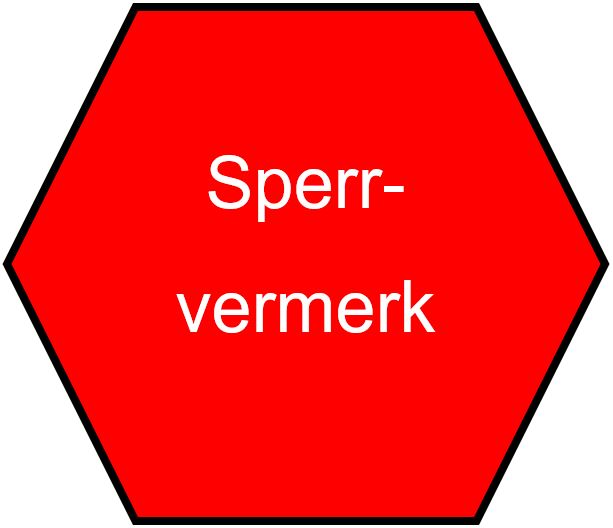
\includegraphics[height=1.5cm]{sperrvermerk.jpg}
	\end{flushright}
	\end{figure}
	\vspace{-5pt}
	\begin{center}
		\vspace{2cm}
		\begin{LARGE}
			\art
			\\
			\vspace{16pt}
		\end{LARGE}
		\begin{Huge}
			\titel
			\\		
			\vspace{14pt}
		\end{Huge}
		\begin{LARGE}
			\untertitel	
		\end{LARGE}
	\end{center}

	\begin{center}
		Fachbereich \studienfach\\
		%Fachrichtung \fachrichtung
		
		An der \hochschule \\ \campus\\
	\end{center}

	\let\stretchbuffer\arraystretch % buffer \arraystretch to restore later
	\renewcommand{\arraystretch}{1} % make table spacing same as line spacing
	\begin{table}[b!]
		\normalsize
		\begin{tabularx}{\textwidth}{lXX}
			\textbf{Eingereicht von:} 				& \textbf{Matrikelnummer:}	& \textbf{Jahrgang} \\
			Ruslan Adilgereev 						& \matrikelnr				& 2023 \\
			Nadine Abu El Komboz					& \matrikelnr				& 2023 \\
			\autor 									& \matrikelnr				& \jahrgang \\

			\\[1cm]
			\textbf{Betreuer:} 	& \gutachter & \\
		\end{tabularx}
	\end{table}
	\renewcommand{\arraystretch}{\stretchbuffer} % restore \arraystretch
	\clearpage
\end{titlepage}


	\section*{Ehrenwörtliche Erklärung}

Hiermit erkläre wir, dass die vorliegende  \art\/ mit dem Thema \newline \newline
{\itshape{} \titel\/}\newline \newline
 selbstständig und ohne fremde Hilfe verfasst
und keine anderen als die angegebenen Quellen und Hilfsmittel benutzt habe. Aus fremden Quellen direkt oder
indirekt übernommene Gedanken habe ich als solche kenntlich gemacht. Die Arbeit habe wir bisher keinem
anderen Prüfungsamt in gleicher oder vergleichbarer Form vorgelegt. Sie wurde bisher auch nicht veröffentlicht.


\vspace{3em}

\abgabeort, \today
\vspace{4em}

\rule{16cm}{0.4pt}\\
Nadine Abu El Komboz \hfill Ruslan Adilgereev \hfill\autor
 

	\pagebreak
	\input{content/Abstract.tex}
	%\include{content/IEEE} % IEEE disclaimer - use with IEEE sources
	%\input{content/Zusammenfassung}
	\pagebreak


	% content lists
	\tableofcontents
	%\lstlistoflistings % list of source code
	\pagebreak

	\pagenumbering{arabic} % start page numbering in arabic

	\chapter{Einleitung}

In der folgenden Dokumentation wird die Implementierung einer Kalender-App beschrieben, mit der Trainingseinheiten gebucht
 werden können. Die Dokumentation erläutert, wie diese Anwendung konzipiert und umgesetzt wurde. Aus der Aufgabenstellung ergaben 
 sich die folgenden Vorgaben für die Bearbeitung:

\begin{itemize}
    \item Anbindung einer Datenbank mittels MariaDB,
    \item Implementierung einer Kalenderjahresansicht,
    \item Farbschema bestehend aus den Farben Blau, Grau und Weiß.
\end{itemize}

Zusätzlich zu diesen vorgegebenen Features konnten noch die folgenden Funktionen integriert werden:

\begin{itemize}
    \item Startseite der App mit allgemeinen Informationen und rechtlichen Hinweisen,
    \item weitere Kalenderansichten (Jahr, Monat, Woche),
    \item Darstellung der Trainingseinheiten in einer Listenansicht (alle Trainings, gebuchte Trainings),
    \item Sortierfunktion für die Listenansichten,
    \item E-Mail-Bestätigung bei der Anmeldung,
    \item Implementierung von Anbieter- und Benutzerrollen:
    \begin{itemize}
        \item Anbieter können Trainings und Trainer hinzufügen,
        \item Benutzer können Trainings buchen.
    \end{itemize}
    \item zusätzliches Farbschema im Dark Mode,
    \item Filterfunktionen (z. B. Suche nach Begriffen und Tags).
\end{itemize}

	\chapter{Aufbau der Software}
	\chapter{Herausforderungen und Lernkurve im Projektverlauf}
Im Verlauf der Projektarbeit traten eine Reihe von praktischen Schwierigkeiten auf, die sowohl technische als auch
konzeptionelle Aspekte betrafen. Zu Beginn gestaltete sich bereits das Einrichten der Entwicklungsumgebung und der 
benötigten Software, insbesondere von MariaDB, als unerwartet aufwändig. Hinzu kam, dass zunächst keinerlei Vorkenntnisse 
in Flutter vorlagen, weshalb eine intensive Einarbeitungsphase erforderlich war, um grundlegende Prinzipien der Flutter-Architektur,
Widgets sowie State-Management zu verstehen und sicher anzuwenden.

Auch auf der UI-Ebene gab es immer wieder komplexe Herausforderungen. Das Darstellen einzelner Interface-Elemente, allen voran die
sogenannte „Training Card“, führte zu unterschiedlichen Fehlerbildern in verschiedenen Ansichten der Anwendung. Parallel dazu 
wuchsen mit fortschreitendem Funktionsumfang die Anforderungen an die Funktionalität: Die Implementierung einer Jahresansicht
für die Trainingskalender, das Hinzufügen effizienter Suchfunktionen und eine flexible Filtermöglichkeit erforderten ein
tiefgreifendes Verständnis der Flutter-Widgets, asynchroner Datenabfragen sowie einer sauberen Trennung von Logik und Darstellung.

Nicht zuletzt stellte auch die Interaktion mit der Datenbank eine anspruchsvolle Aufgabe dar. Der Aufbau performanter,
sicherer und gleichzeitig wartungsfreundlicher Datenbankabfragen sowie die Koppelung an die Frontend-Logik verlangten
sowohl Sorgfalt als auch ein gewisses Maß an Trial-and-Error. Diese Erfahrungen führten letztlich zu einem enormen Lernzuwachs,
stärkten das Verständnis für die gesamtheitliche Systemarchitektur und halfen dabei, künftige Herausforderungen systematischer
und effizienter anzugehen.
	\chapter{Testing}

Um die Kalender-App zu testen, wurden zwei Arten von Tests durchgeführt: Widget-Tests und Unit-Tests.

\section{Unit-Test}

Mithilfe eines Unit-Tests können einzelne Methoden und Funktionen überprüft werden. Im Test werden die erforderlichen 
Eingabeparameter simuliert und die Ausgabeparameter auf ihre Korrektheit hin überprüft. Ein Unit-Test greift während der 
Testdurchführung nicht auf die Festplatte zu. Dadurch werden weder Grafiken gerendert noch Benutzereingaben berücksichtigt.

Unit-Tests dienen daher ausschließlich dazu, die Logik einzelner Methoden zu überprüfen. Sie eignen sich jedoch nicht, um die
 Schnittstellenfunktionalität oder die Interaktion mit Benutzern zu testen.

\section{Widget-Test}
Der Widget-Test wird verwendet, um die Interaktion mit dem Benutzer und die grafische Darstellung der App zu überprüfen. In einer 
isolierten Testumgebung werden Widgets erzeugt und getestet, ob sie korrekt gerendert wurden. Darüber hinaus wird überprüft, 
ob Benutzereingaben korrekt verarbeitet werden und das erneute Rendering der Benutzeroberfläche ordnungsgemäß funktioniert.

\section{Implementierung}

Es wurden zwei Arten von Tests implementiert, um die Funktionalität der Kalender-App sicherzustellen:
\begin{itemize}
    \item Unit-Tests, um die Logik einzelner Methoden innerhalb von Flutter zu überprüfen.
    \item Widget-Tests, um die Benutzerinteraktion und die korrekte grafische Darstellung der Anwendung zu validieren.
\end{itemize}

Der Code für die Testprogramme wurde in den folgenden Dateien umgesetzt: \textit{"training\_service\_test.dart"},
 \textit{"training\_service\_test.mocks.dart"} und \textit{"widget\_test.dart"}.
Bei \textit{"training\_service\_test.dart"} und der Datei \textit{"training\_service\_test.mocks.dart"} handelt es sich
um den Unit-Test, wobei die Datei \textit{"training\_service\_test.mocks.dart"} eine Simulationsumgebung umsetzt und die andere Datei
 den eigentlichen Test enthält.
Durch die begrenzte Zeit wurde jeder Test jeweils für eine Methode implementiert. Mittels des Unit-Tests wurde die Funktion der
 Trainingssuche getestet. Dabei wurden die folgenden vier Szenarien betrachtet:
\begin{itemize}
    \item Erfolgreiche Antworten (gültige Trainingsdaten).
    \item Fehlerhafte Antworten (Fehlerstatus oder ungültige JSON-Daten).
    \item Leere Antworten (keine Trainings gefunden).
    \item Formatierung von null-Werten oder fehlenden Daten.
\end{itemize}

Beim Widget-Test wurde die ordnungsgemäße Initialisierung der \textit{ThemeService}- und \textit{AuthService}-Provider getestet. 
Das Ergebnis des Testprotokolls befindet sich im Anhang.



	\input{content/BenötigteSoftware.tex}
	\chapter{Bedinung des Benutzers}


	\chapter{Fazit und Ausblick}


	
	\renewcommand{\refname}{Literaturverzeichnis}
	%Literaturverzeichnis einfügen
	\printbibliography
%	\pagebreak
	\appendix
	\chapter{Anhang}
\label{Anhang}

\section{Inhalte der CD}
\label{CD}
    \begin{itemize}
        \item \LaTeX-Dateien der \art
        \item nichtöffentliche Quellen
        \item sämtliche verwendete Grafiken
    \end{itemize}

    %\section{Zusätzliche Grafiken}
    \section{Zusätzliche Berechnungen}



\end{document}